%! Author = breandanconsidine
%! Date = 7/19/21

% Preamble
\documentclass[mathserif,notheorems]{beamer}

% Packages
\usepackage{fontspec}
\usepackage{amsmath}

% https://tex.stackexchange.com/a/34486/139648
\usepackage{tikz}
\usetikzlibrary{calc}
\newcommand{\tikzmark}[1]{\tikz[overlay,remember picture] \node (#1) {};}

\usepackage[pdf]{graphviz}
\usepackage{amssymb}
\usepackage{mathrsfs}
\usepackage{xcolor}
\usepackage{pifont}% http://ctan.org/pkg/pifont
\newcommand{\cmark}{\color{green}\ding{51}}%
\newcommand{\xmark}{\color{red}\ding{55}}%
\usepackage{multicol}

\usepackage[normalem]{ulem}

\usepackage{blkarray}% http://www.hss.caltech.edu/~kcb/TeX/kbordermatrix.sty
\makeatletter
\def\squiggly{\bgroup \markoverwith{\textcolor{red}{\lower3\p@\hbox{\sixly \char58}}}\ULon}
\makeatother

\newcommand{\err}[1]{\smash{\squiggly{#1}{}}}


% https://tex.stackexchange.com/a/285558/139648
\usepackage{amsthm}
\setbeamertemplate{theorems}[numbered] % to number

\theoremstyle{plain} % insert bellow all blocks you want in italic
\newtheorem{theorem}{Theorem}[section] % to number according to section

\theoremstyle{definition} % insert bellow all blocks you want in normal text
\newtheorem*{definition}{Definition} % to number according to section
\newtheorem*{idea}{Proof idea} % no numbered block

\usepackage{graphicx}
\usepackage{tcolorbox}
% ---------

\title{Interactive Programming\\ with Automated Reasoning}
\author{Breandan Considine}

\institute[McGill]{
  McGill University \\
  \medskip
  \textit{breandan.considine@mail.mcgill.ca}
}
\date{\today}

% Document
\begin{document}
\begin{frame}
  \titlepage
\end{frame}

%\begin{frame}
%  \frametitle{Programming as a tool for thought}
%  \begin{tcolorbox}
%    There is a race between the increasing
%    complexity of the systems we build and our
%    ability to develop intellectual tools for
%    understanding their complexity.
%    If the race is won by our tools, then
%    systems will eventually become easier to
%    use and more reliable. If not, they will
%    continue to become harder to use and less
%    reliable for all but a relatively small
%    set of common tasks.
%    Given how hard thinking is, if those
%    intellectual tools are to succeed,
%    they will have to substitute calculation
%    for thought.
%    \begin{flushright}
%      --Leslie Lamport
%    \end{flushright}
%  \end{tcolorbox}
%\end{frame}

\begin{frame}
  \frametitle{Research Interests}
  How do we use software to build more intelligent systems, and how can we use intelligent systems to help us write better software?\vspace{10pt}

  Find programmer friction points, formalize them as optimization problems, solve and publish our solutions as new developer tools.

  \vspace{10pt}
  \begin{itemize}
    \item Realtime developer assistance
    \item Code completion and program repair
    \item Documentation search and retrieval
    \item Editing and refactoring source code
    \item Assistance for impaired developers
  \end{itemize}
  \vspace{10pt}

  Important: build tools that we personally need or want to use, then \textit{use} the tools we built to identify and improve usability issues.
\end{frame}

\begin{frame}
  \frametitle{Tools for assistive programming}
  Three developer tools and their core optimization problems:\vspace{10pt}

  \begin{itemize}
    \item \textbf{AceJump} - A single character search, select, and jump
    \begin{itemize}\item Minimizes finger travel distance in keyboard navigation\end{itemize}
    \item \textbf{Tidyparse} - Syntax repair for programming languages
    \begin{itemize}\item Minimizes Levenshtein edit distance subject to a grammar\end{itemize}
    \item \textbf{Idiolect} - Handsfree audio development interface
    \begin{itemize}\item Minimizes intent-recognition failures in voice programming\end{itemize}
  \end{itemize}
  \vspace{10pt}
  \begin{center}
\includegraphics[scale=0.20]{icons}\end{center}
\end{frame}

\begin{frame}
  \frametitle{Tag Assignment in AceJump}
  Helps developers search and navigate code rapidly. To do so, we solve the \textbf{Tag Assignment Problem}, i.e., stated formally:

\vspace{10pt}
  Given a set of indices $I$ in document $d$, and a set of tags $T$, find a bijection $f: T^*\subset T \leftrightarrow I^*\subset I$, maximizing $|I^*|$, such that:

  \begin{equation*}
    d[i\ldots k] + t \notin d[i'\ldots(k + |t|)], \forall i' \in I\setminus\{i\}, \forall k \in (i, |d| - |t|]
  \end{equation*}

 where $t \in T, i \in I$. This can be relaxed to $t=t[0]$ and $\forall k \in (i, i+K]$ for some fixed $K$, in most natural documents.

  \vspace{10pt}
  \textbf{Natural language:}
  \textit{Maximizes the number of non-conflicting tags assigned to search results in uniquely-selectable manner, i.e., should never be possible to select a tag by mistake.}
\end{frame}

\begin{frame}
  \frametitle{AceJump Usage}
  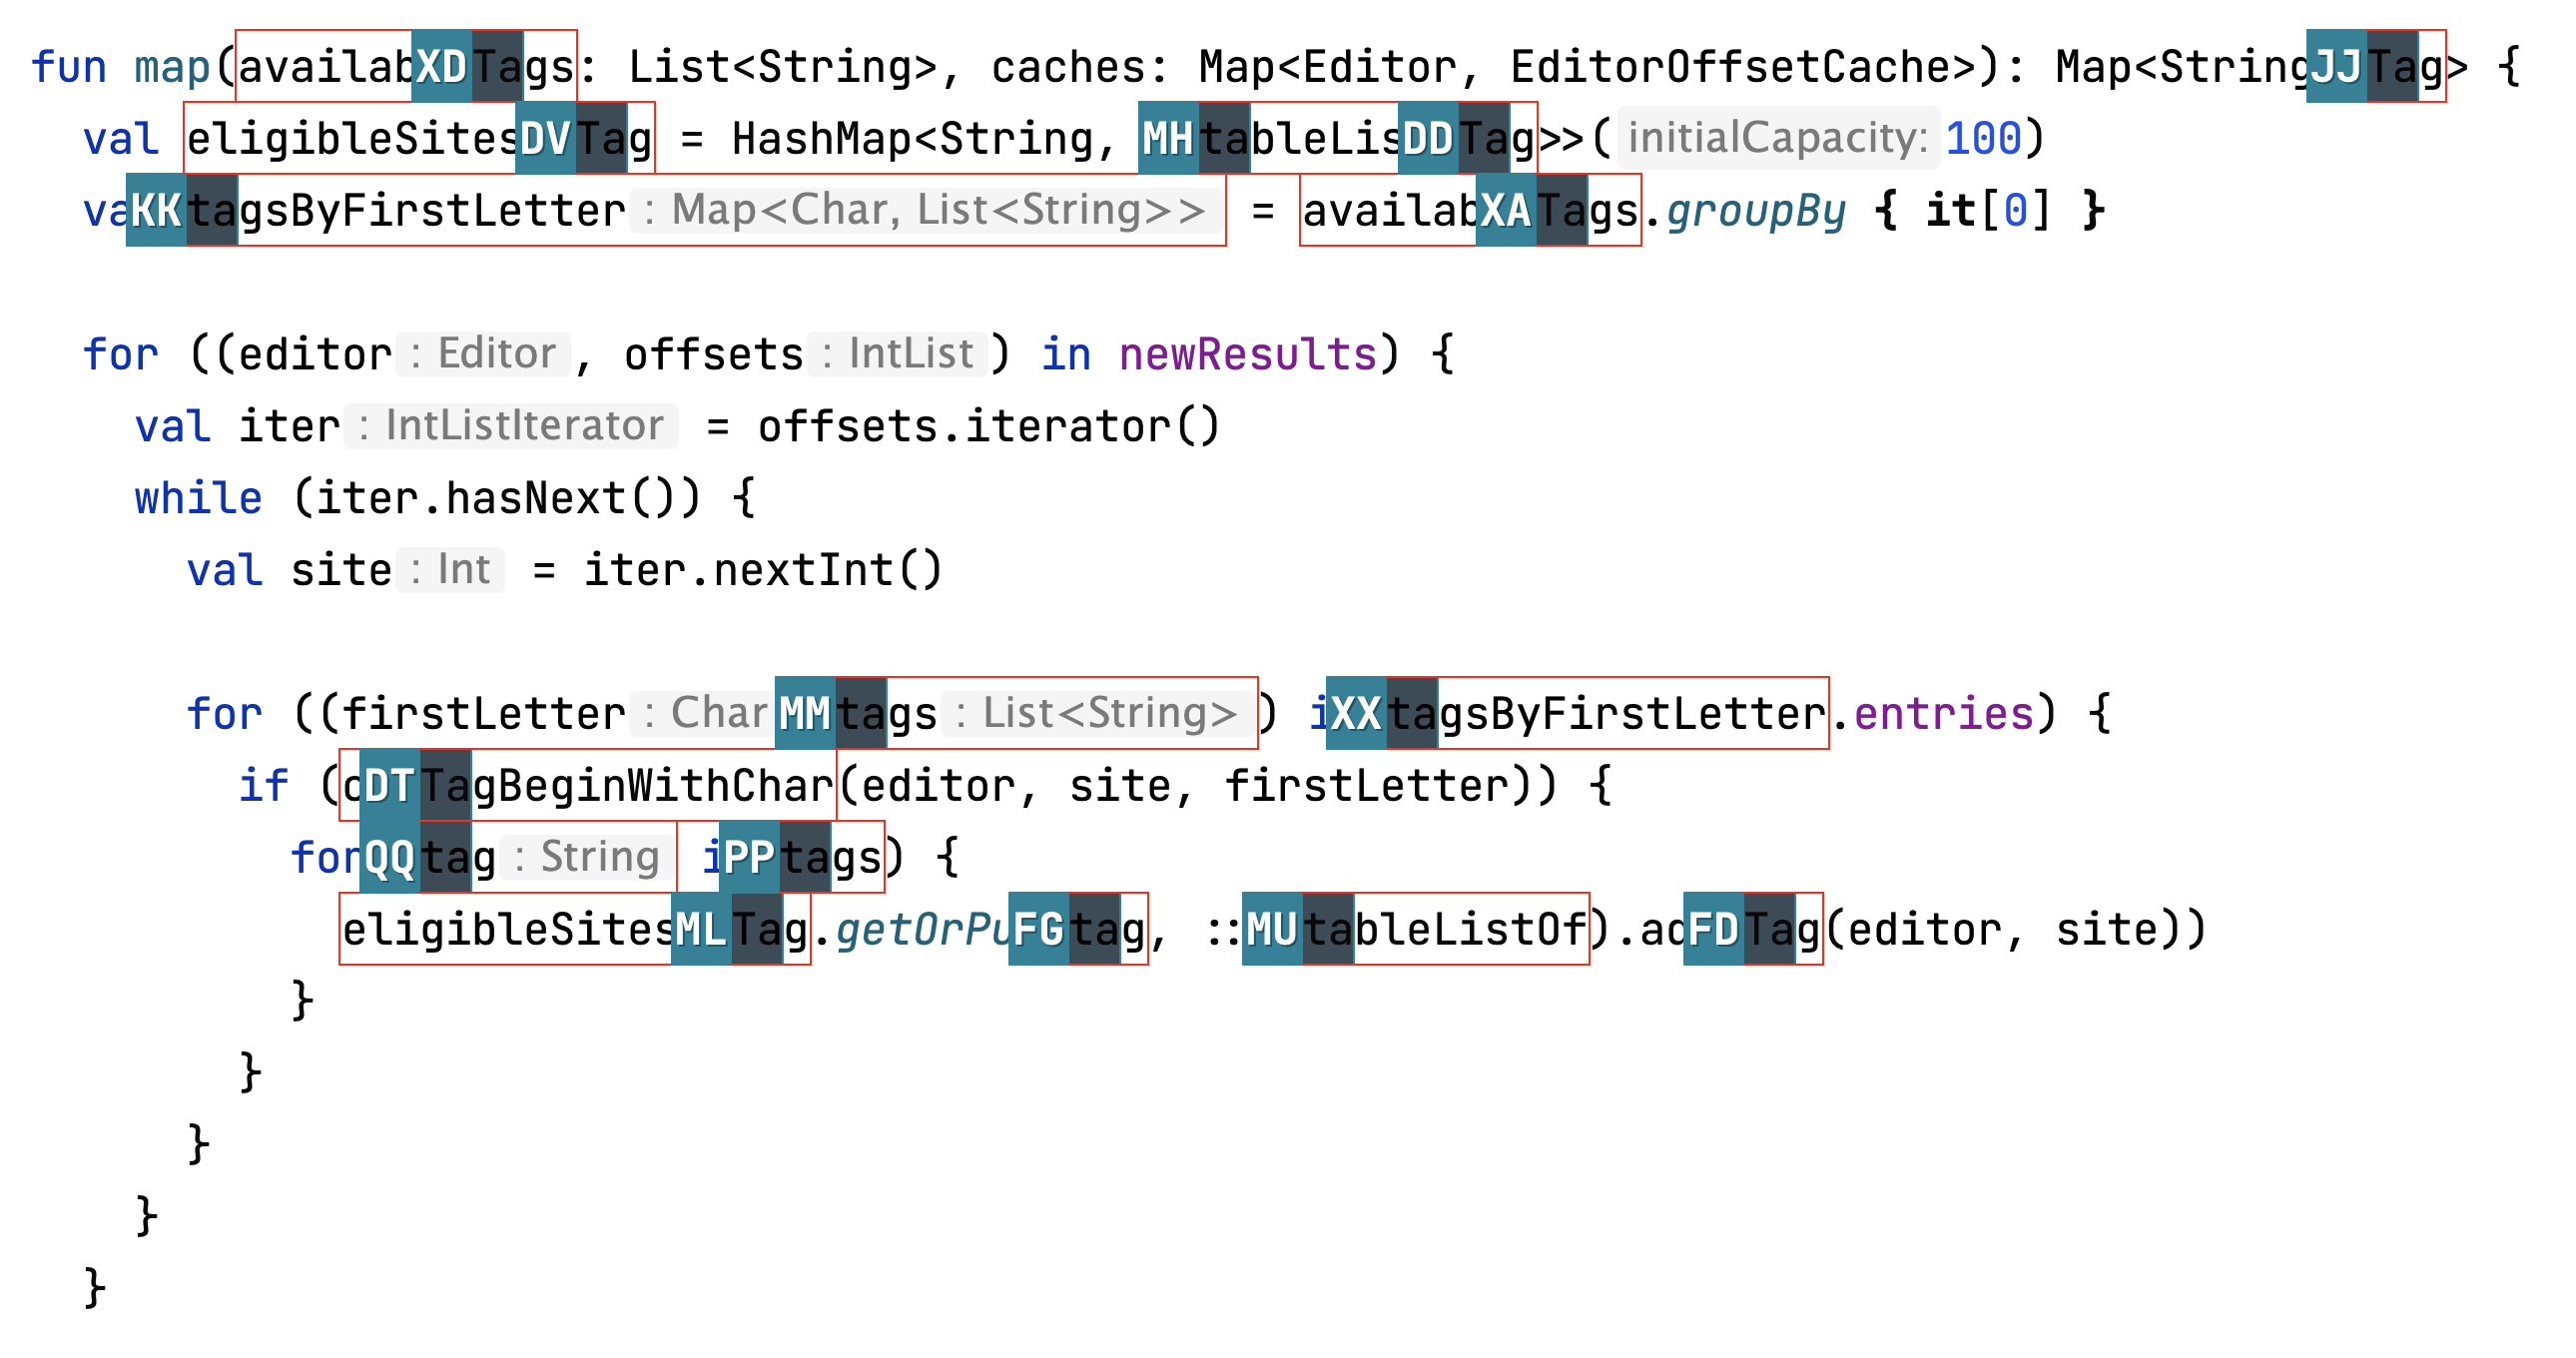
\includegraphics[scale=0.25]{acejump_screenshot}
\end{frame}

\begin{frame}
  \frametitle{AceJump Adoption}
  $\sim 7\times 10^5$ downloads, $\sim 10^4$ monthly active users, $\sim 10^3$ stars.\vspace{20pt}
  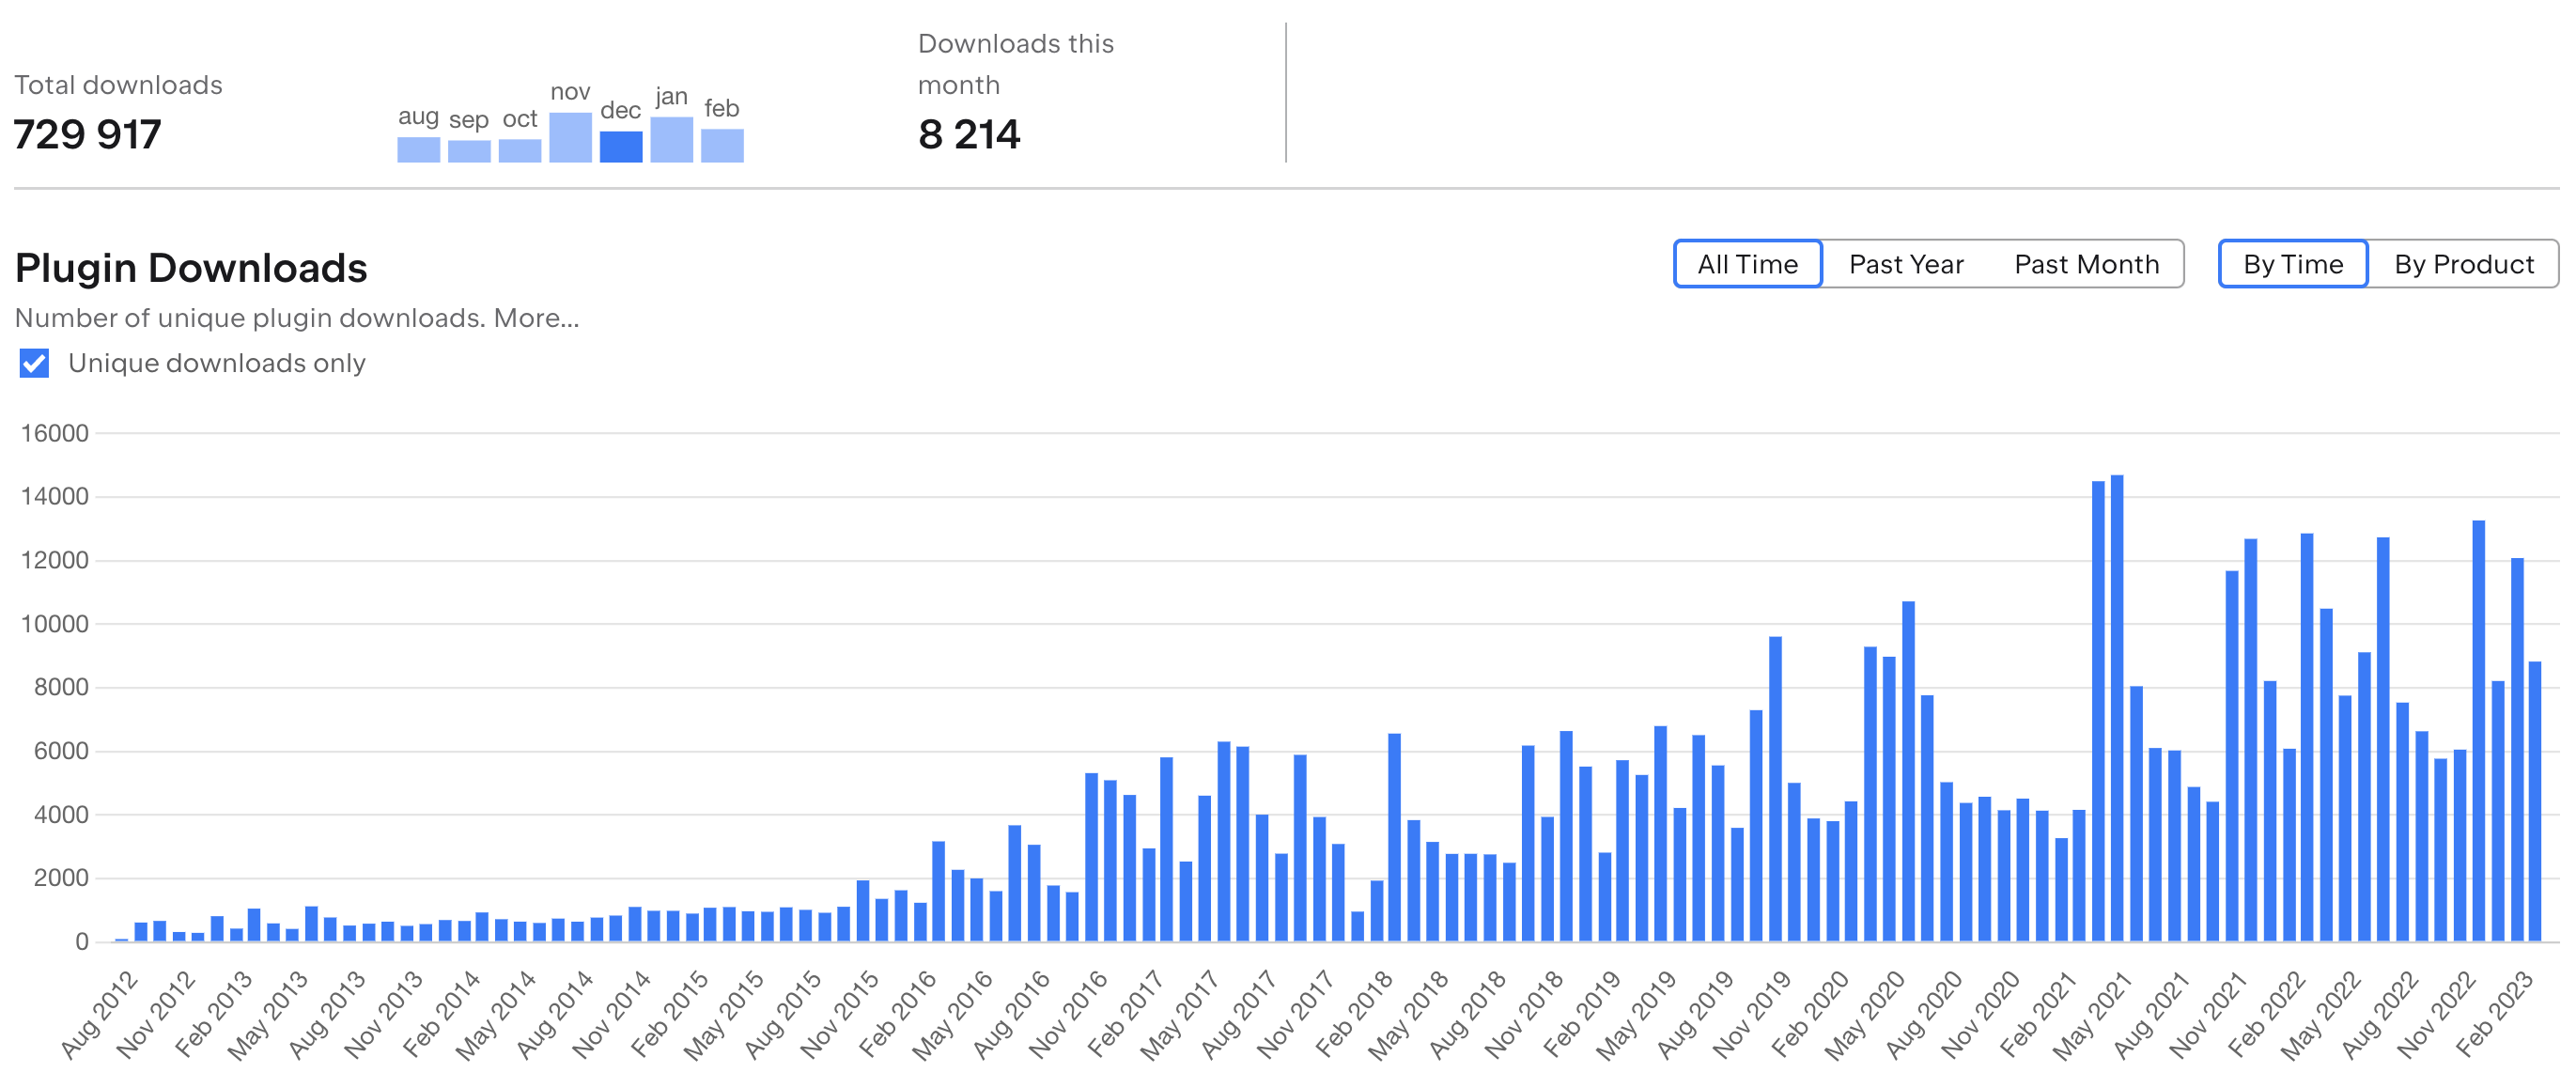
\includegraphics[scale=0.22]{acejump_adoption}
\end{frame}

\begin{frame}
  \frametitle{Error Correction in Tidyparse}
  Helps novice programmers fix syntax errors in source code. We do so by solving the \textbf{Bounded Levenshtein Reachability Problem}:\vspace{10pt}

Given a conjunctive grammar $\mathcal{G}$, a fixed edit distance $r$, and a malformed string $\err{\sigma}: \Sigma^*$, find all syntactically well-formed strings $\{\tilde{\sigma} \in \mathcal{L}(\mathcal{G}) \mid \Delta(\err{\sigma}, \tilde{\sigma}) < r\}$, ranked by Levenshtein edit distance.

  \begin{center}
  \resizebox{0.4\textwidth}{!}{
    \begin{tikzpicture}[
      dot/.style = {circle, inner sep=0pt, minimum size=1mm, fill,
      node contents={}}
    ]
      \def\firstcircle{(-2.1,0) coordinate (a) circle (2.4cm)}
      \def\firstcirclea{(-2.1,0) coordinate (b) circle (0.6cm)}
      \def\firstcircleb{(-2.1,0) coordinate (c) circle (1.2cm)}
      \def\firstcirclec{(-2.1,0) coordinate (d) circle (1.8cm)}
      \def\secondcircle{(1.2,0) coordinate (e) circle (1.5cm)}
      \begin{scope}
        \clip \secondcircle;
        \fill[black!15] \firstcircle;
      \end{scope}
      \draw \firstcircle node[dot,label=$\err{\sigma}$](z0);
      \draw [dashed] \firstcirclea;
      \draw [dashed] \firstcircleb;
      \draw [dashed] \firstcirclec;
      \draw[-stealth] (-2.1,0) -- (-1.5, 0) node[midway,below]{$d_1$};
      \draw[-stealth] (-1.5,0) -- (-0.9, 0) node[midway,below]{$d_2$};
      \draw[-stealth] (-0.9,0) -- (-0.3, 0) node[midway,below]{$\vphantom{d}\ldots$};
      \draw[-stealth] (-0.3,0) -- (0.3, 0) node[midway,below]{$d^*$};
      \draw[-stealth] (-0.3,0) -- (0.3, 0) node[midway,above]{$\tilde{\sigma}$};
      \draw \secondcircle;
      \node [above] at (current bounding box.north -| a) {$\mathcal{L}(G(\err\sigma, r^*))$};
      \node [above,yshift=1.5cm] at (e) {$\mathcal{L}(\mathcal{G})$};
    \end{tikzpicture}
  }
  \end{center}



  \textbf{Natural language:}
  \textit{Finds all syntactically valid repairs within a small edit distance, ranked by similarity to the original input.}
\end{frame}

\begin{frame}
  \frametitle{Tidyparse Usage}
  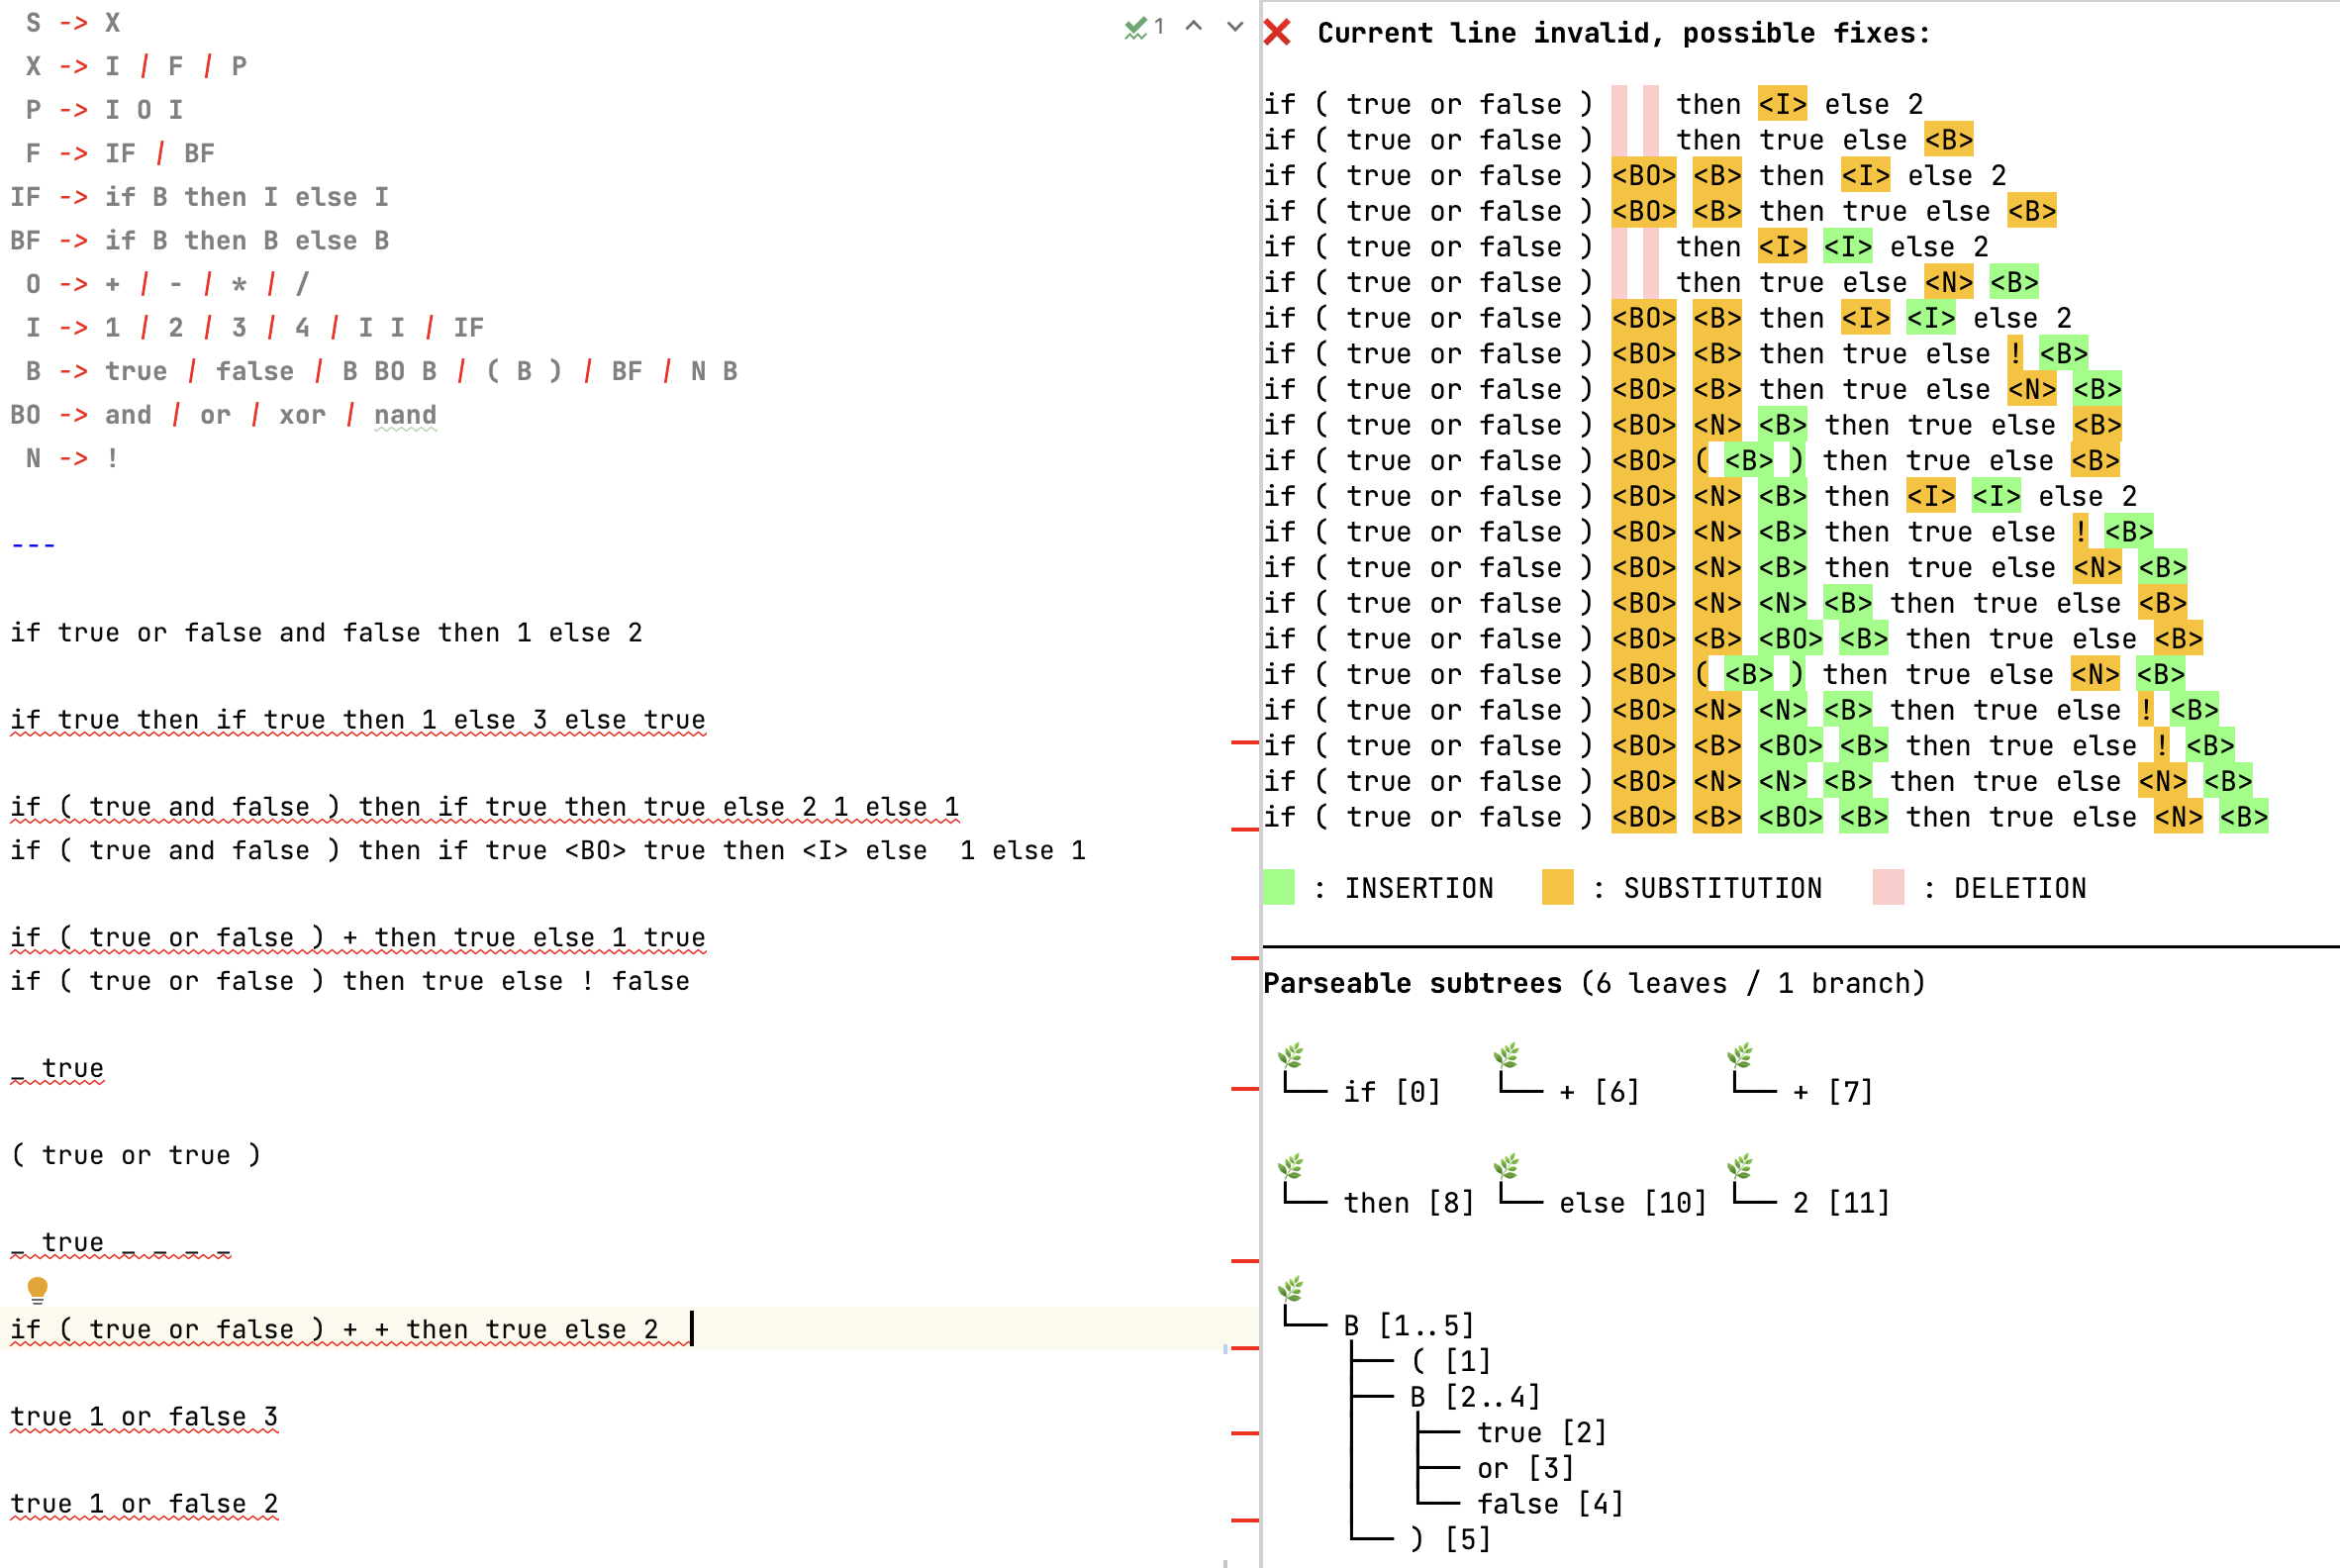
\includegraphics[scale=0.25]{tidyparse_screenshot}
\end{frame}

\begin{frame}
  \frametitle{Intent Recognition in Idiolect}
  Helps programmers with motor and visual impairments write code. We do so by solving the \textbf{IDE-intent recognition problem}:\vspace{10pt}

  Given an audio signal containing an arbitrary stream of words, $S(\Sigma) = 1 + \Sigma\cdot S(\Sigma)$ consisting of subsequences from a context-free grammar find the optimal alignment of non-overlapping commands from that grammar satisfying the given command.\vspace{10pt}

  \textbf{Natural language:}
  \textit{Given a series of spoken voice commands, find the optimal alignment of actions satisfying the user's intent.}

\end{frame}

\begin{frame}
  \frametitle{Idiolect Overview}
  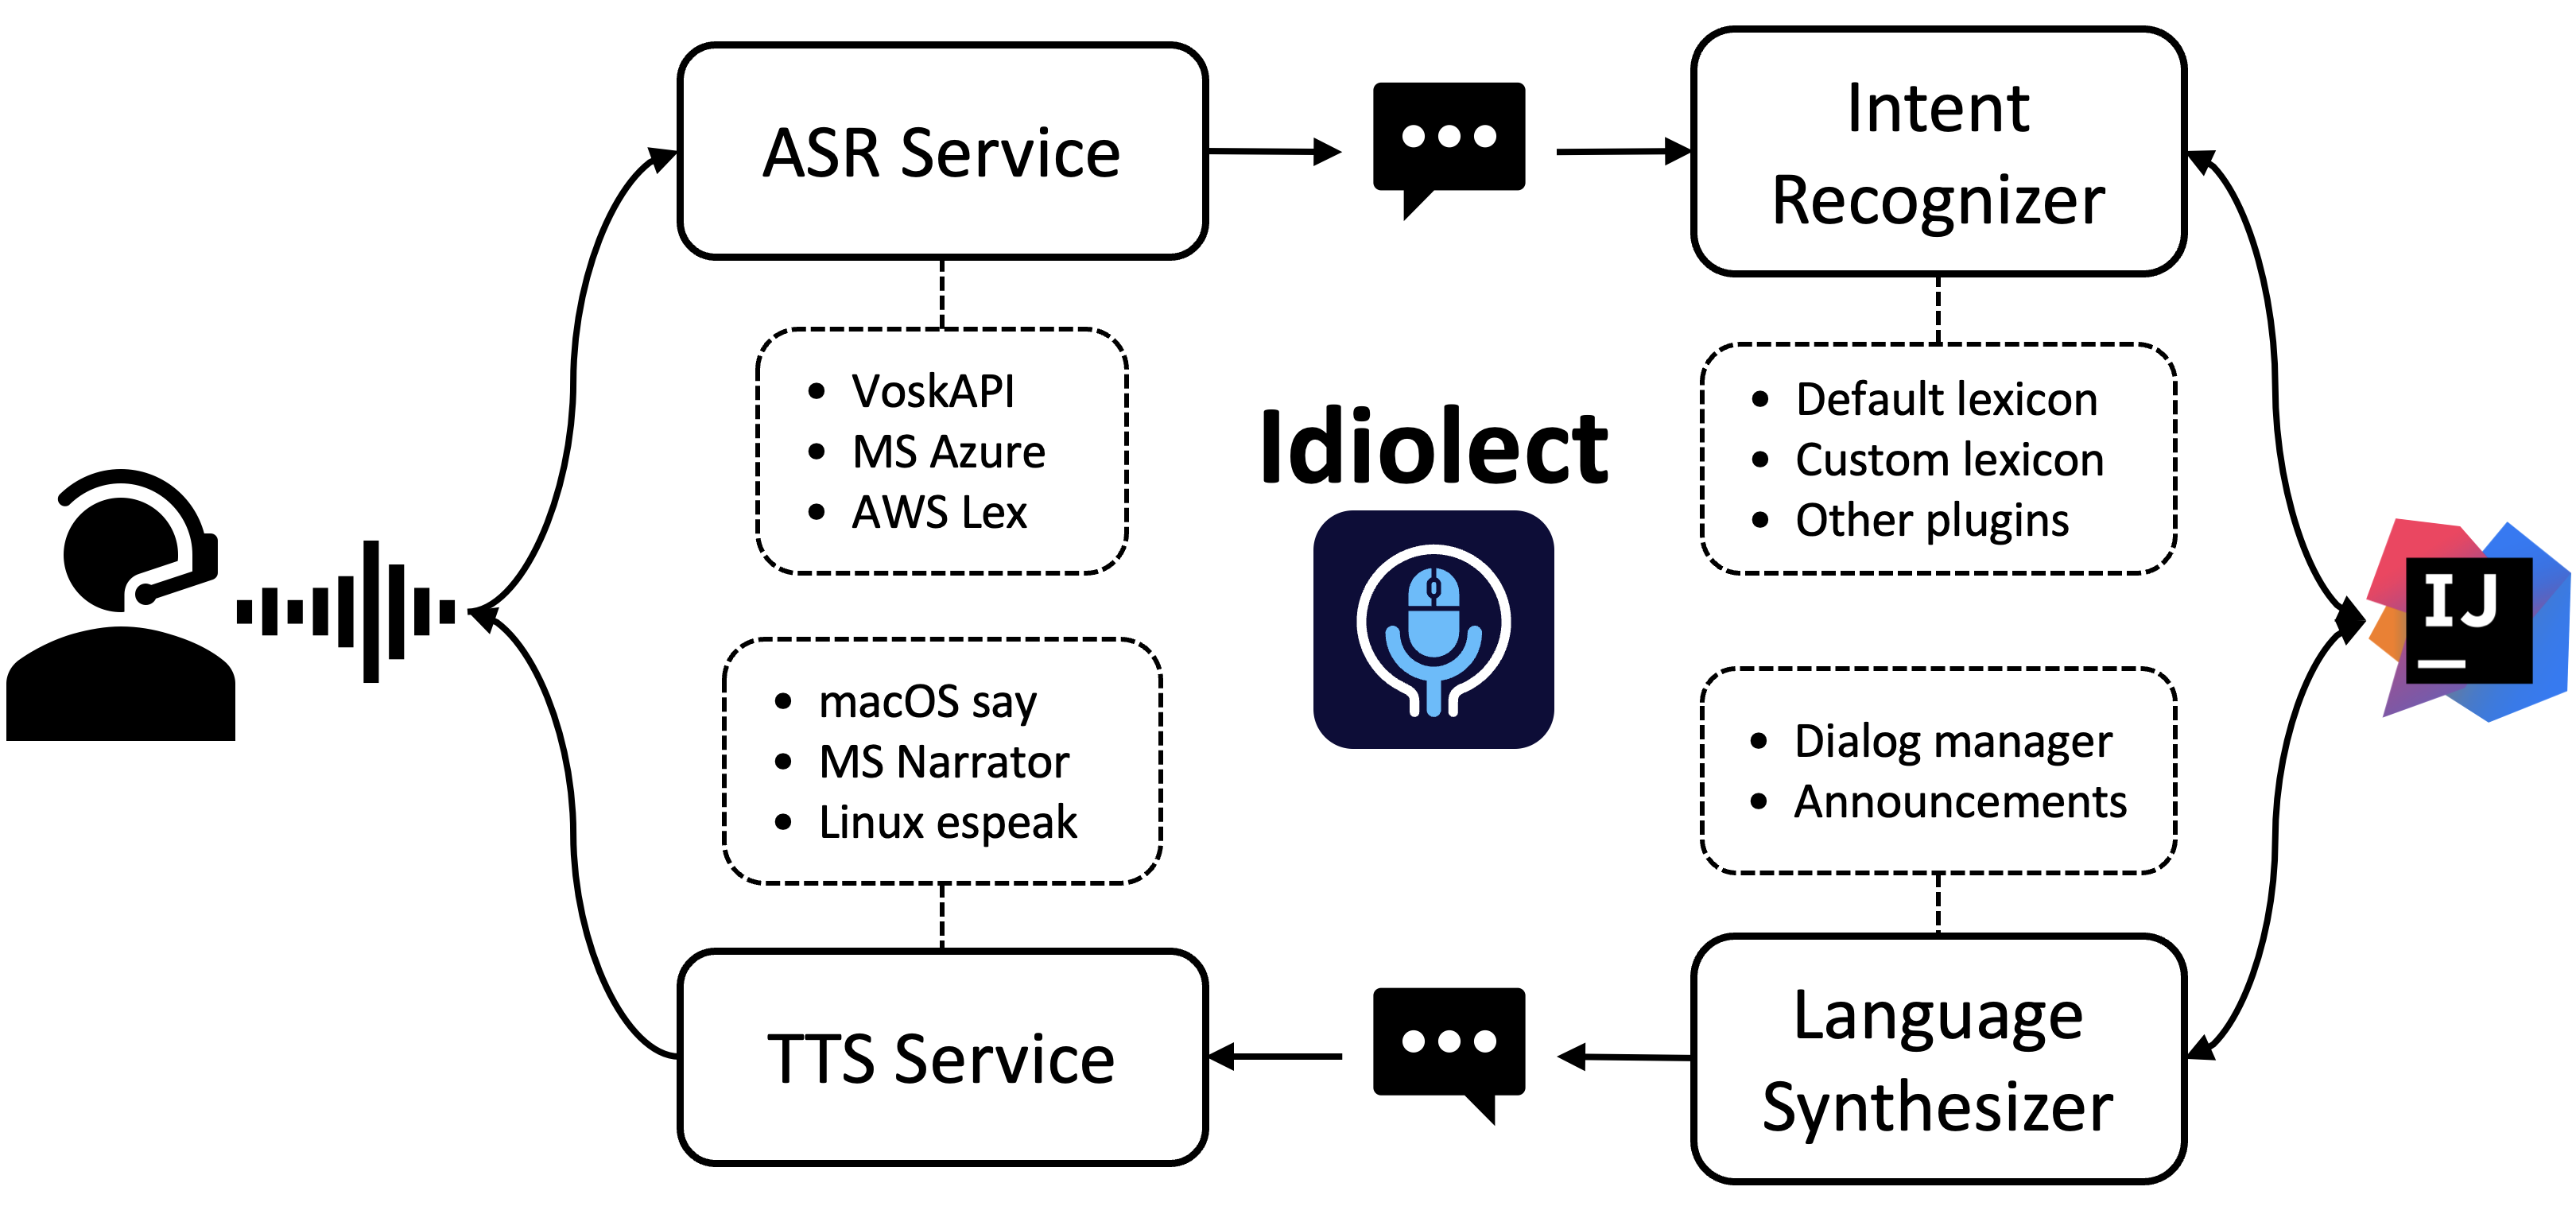
\includegraphics[scale=0.185]{idiolect_overview}
\end{frame}

\begin{frame}
  \frametitle{Research Summary}
  My research studies:
  \begin{itemize}
  \item Information foraging patterns in software development
  \item Common programming mistakes and their solutions
  \item Usability and accessibility challenges in programming
  \end{itemize}\vspace{10pt}
  Using the insights gained, we:
  \begin{itemize}
  \item Reframe usability issues as optimization problems
  \item Formalize and solve those problems using pen and paper
  \item Integrate the solutions into real-world developer tools
  \end{itemize}\vspace{10pt}
  This helps developers be more productive by providing:
  \begin{itemize}
  \item More contextually-aware user interfaces
  \item Safer and more flexible code completion
  \item More accessible and interactive developer tools
  \end{itemize}
\end{frame}

\begin{frame}
  \frametitle{Acknowledgements}
  \textbf{Academic Advisors}
  \begin{multicols}{2}
    \begin{itemize}
      \item \href{https://www.cs.mcgill.ca/~jguo/}{Jin Guo}
      \item \href{https://www.cs.toronto.edu/~six/}{Xujie Si}
      \end{itemize}
  \end{multicols}
  \textbf{Collaborators/Contributors}
  \begin{multicols}{2}
    \begin{itemize}
      \item \href{https://github.com/nalbion}{Nicholas Albion}
      \item \href{https://chylex.com/}{Daniel Ch\'ylek}
      \item \href{https://github.com/AlexPl292}{Alex Pl\'ate}
      \item \href{https://johnlindquist.com/}{John Lindquist}
      \item \href{https://github.com/alexeykudinkin}{Alexey Kudinkin}
      \item \href{https://github.com/lepenkinya}{Yaroslav Lepenkin}
    \end{itemize}
  \end{multicols}
  \textbf{Feedback/Inspiration}
  \begin{multicols}{2}
    \begin{itemize}
      \item \href{https://www.iro.umontreal.ca/~monnier/}{Stefan Monnier}
      \item \href{https://www.cs.mcgill.ca/~bpientka/}{Brigitte Pientka}
      \item \href{https://tscholak.github.io/}{Torsten Scholak}
      \item \href{https://people.csail.mit.edu/jcito/}{J\"urgen Cito}
      \item \href{https://mcschroeder.github.io/}{Michael Schr\"oder}
      \item \href{https://oriroth.github.io/}{Ori Roth}
      \item \href{https://younesse.net/}{Younesse Kaddar}
      \item \href{https://gopiandcode.uk/}{Kiran Gopinathan}
    \end{itemize}
  \end{multicols}
\end{frame}

\end{document}

